% \begin{figure*}
% \centering
%     \begin{subfigure}{0.54\textwidth}
%         \centering
%         \includegraphics[width=\textwidth]{chapters/uotod/image/draft_OT_matching_illustration.png}
%         \label{fig:}
%         \caption{DRAFT/SKETCH illustration}
%     \end{subfigure}
%     \hfill
%     \begin{subfigure}{0.45\textwidth}
%         \centering
%         \includesvg[pretex=\footnotesize, width=\textwidth]{chapters/uotod/image/mAP_DETR_color-H_balanced.svg}
%         \label{fig:DETR-toy-balanced-mAP}
%         \caption{}
%     \end{subfigure}
%     \label{fig:}
%     \caption{CAPTION TO WRITE}
% \end{figure*}

\begin{figure}
    \centering
    % \captionsetup{justification=justify}
    \begin{tabular}[t]{ccc}
    \multicolumn{2}{c}{%
    % \subcaptionbox{Image \textnumero 163 from the COCO training dataset. The ground truths are colored and fictive predictions are outlined in black.%
    %     \label{fig:general-img}}[.30\textwidth]%
    %     {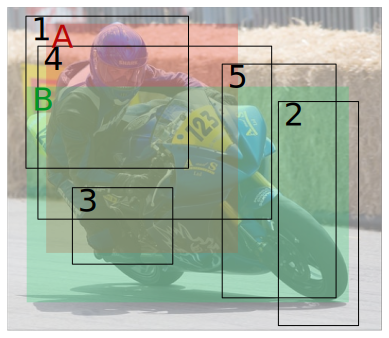
\includegraphics[width=.29\textwidth]{chapters/uotod/image/general/img.png}}}%
    \begin{subfigure}{0.6\textwidth}
        \centering
        %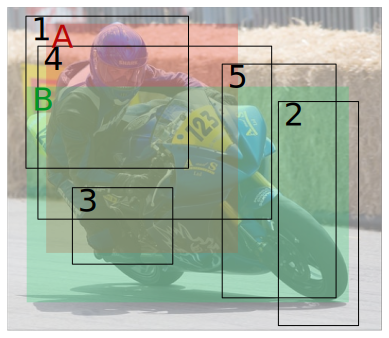
\includegraphics[width=\textwidth]{chapters/uotod/image/general/img.png}
        \def\svgwidth{.7\textwidth}\footnotesize
        \import{chapters/uotod/image/general}{img.pdf_tex} 
        \caption{Image \textnumero 163 from the VOC training dataset. The ground truth boxes are colored, and the predictions are outlined in black.%
        \label{fig:general-img}}
    \end{subfigure}}%
    &
    \begin{subfigure}{.3\textwidth}
        \centering \footnotesize
        %\includesvg[pretex=\footnotesize,width=1.13\textwidth]{chapters/uotod/image/general/cost.svg}
        \def\svgwidth{0.6\textwidth}
        \import{chapters/uotod/image/general}{cost.pdf_tex}
        \caption{Costs between the predictions and the ground truth ($1-\mathrm{GIoU}$). The background cost is $c_{\varnothing} = 0.8$.%
        \label{fig:general-cost}}
    \end{subfigure}\\%
    % &\subcaptionbox{Costs between the predictions and the ground truths ($1-\mathrm{GIoU}$). The background cost is $c_{\varnothing} = 0.8$.%
    %     \label{fig:general-cost}}[.13\textwidth]%
    %     {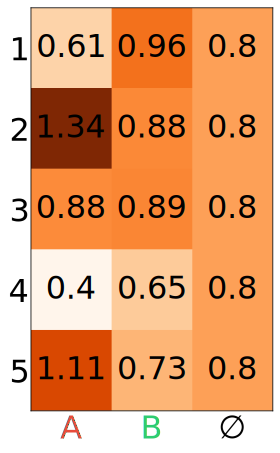
\includegraphics[width=.12\textwidth]{chapters/uotod/image/general/cost.png}}\\%
    \subcaptionbox{Prediction to best ground truth (\gls{uot} with $\epsilon=0$, $\tau_1\rightarrow+\infty$ and $\tau_2=0$).%
        \label{fig:general-min1}}[.3\textwidth]%
        {\centering \footnotesize
        %\includesvg[pretex=\footnotesize,width=.148\textwidth]{chapters/uotod/image/general/min1.svg}
        \def\svgwidth{.18\textwidth}
        \import{chapters/uotod/image/general}{min1.pdf_tex}
        }%
    &%
    \subcaptionbox{Hungarian matching (\gls{ot} with $\epsilon=0$, $\tau_1 \rightarrow +\infty$ and $\tau_2 \rightarrow + \infty$).%
        \label{fig:general-hungarian}}[.3\textwidth]%
        {\centering \footnotesize
        %\includesvg[pretex=\footnotesize,width=.148\textwidth]{chapters/uotod/image/general/hungarian.svg}
        \def\svgwidth{.18\textwidth}
        \import{chapters/uotod/image/general}{hungarian.pdf_tex}
        }%
    &%
    \subcaptionbox{Ground truth to best prediction (\gls{uot} with $\epsilon=0$, $\tau_1 = 0 $ and $\tau_2 \rightarrow +\infty$).%
        \label{fig:general-min2}}[.3\textwidth]%
        {\centering \footnotesize
        %\includesvg[pretex=\footnotesize,width=.148\textwidth]{chapters/uotod/image/general/min2.svg}
        \def\svgwidth{.18\textwidth}
        \import{chapters/uotod/image/general}{min2.pdf_tex}
        }%
    \\
    \subcaptionbox{\gls{uot} with $\epsilon = 0.05$, $\tau_1=100$ and $\tau_2=0.01$.%
        \label{fig:general-unb1}}[.3\textwidth]%
        {\centering \footnotesize
        %\includesvg[pretex=\footnotesize,width=.148\textwidth]{chapters/uotod/image/general/unb1.svg}
        \def\svgwidth{.18\textwidth}
        \import{chapters/uotod/image/general}{unb1.pdf_tex}
        }%
    &%
    \subcaptionbox{\gls{ot} with $\epsilon=0.05$ ($\tau_1 \rightarrow +\infty$ and $\tau_2 \rightarrow +\infty$).%
        \label{fig:general-reg}}[.3\textwidth]%
        {\centering \footnotesize
        %\includesvg[pretex=\footnotesize,width=.148\textwidth]{chapters/uotod/image/general/reg.svg}
        \def\svgwidth{.18\textwidth}
        \import{chapters/uotod/image/general}{reg.pdf_tex}
        }%
    &%
    \subcaptionbox{\gls{uot} with $\epsilon = 0.05$, $\tau_1=0.01$ and $\tau_2=100$.%
        \label{fig:general-unb2}}[.3\textwidth]%
        {\centering \footnotesize
        %\includesvg[pretex=\footnotesize,width=.148\textwidth]{chapters/uotod/image/general/unb2.svg}
        \def\svgwidth{.18\textwidth}
        \import{chapters/uotod/image/general}{unb2.pdf_tex}
        }%
    \end{tabular}
    \caption{Different matching strategies. All are particular cases of \emph{Unbalanced Optimal Transport}. A match ($\hat{P}_{i,j}=1$) is denoted by a black square and it is white if there is no match ($\hat{P}_{i,j}=0$).}%
    \label{fig:general}
    \vspace{-2em}
\end{figure}

\section{Introduction}
Object detection models are in essence multi-task models, having to both localize objects in an image and classify them. In the context of supervised learning, each of these tasks heavily depends on a matching strategy. Indeed, determining which predicted object matches which ground truth object is a non-trivial yet essential task during the training (Figure~\ref{fig:general-img}). In particular, the matching strategy must ensure that there is ideally exactly one prediction per ground truth object, at least during inference. Various strategies have emerged, often relying on hand-crafted components. They are proposed as scattered approaches that seem to have nothing in common, at least at first glance. 

\subsection{A Unifying Framework}
To perform any match, a matching cost has to be determined. The example at Fig.~\ref{fig:general-cost} uses the \emph{Generalized Intersection over Union} ($\mathrm{GIoU}$)~\cite{giou}. Given such a cost matrix, matching strategies include:

\begin{itemize}
    \item Matching each prediction to the closest ground truth object. This often requires that the cost lies under a certain threshold~\cite{liu2016ssd,ren2015fasterrcnn,redmon2016yolo,lin2017focalloss}, to avoid matching predictions that may be totally irrelevant for the current image. The disadvantage of this strategy is its redundancy: many predictions may point towards the same ground truth object. In Fig.~\ref{fig:general-min1}, both predictions 1 and 4 are matched towards ground truth object \textcolor{red}{A}. Furthermore, some ground truth objects may be unmatched. A solution to this is to increase the number of predicted boxes drastically. This is typically the case with anchors boxes and region proposal methods.
    
    \item The opposite strategy is to match each ground truth object to the best prediction~\cite{he2015spatial,liu2016ssd}. This ensures that there is no redundancy and every ground truth object is matched. This also comes with the opposite problem: multiple ground truth objects may be matched to the same prediction. In Fig.~\ref{fig:general-min2}, both ground truth objects \textcolor{red}{A} and \textcolor{green}{B} are matched to prediction 4. This can be mitigated by having more predictions, but then many of those are left unmatched, slowing convergence~\cite{liu2016ssd}.
    
    \item A compromise is to perform a \emph{Bipartite Matching} (BM), using the \emph{Hungarian algorithm}~\cite{kuhn1955hungarian,munkres1957algorithmstransportationhungarian}, for example~\cite{carion2020detr,zhu2020deformabledetr}. The matching is one-to-one, minimizing the total cost (Definition~\ref{def:lap}). Every ground truth object is matched to a unique prediction, thus reducing the number of predictions needed, as shown in Fig.~\ref{fig:general-hungarian}. A downside is that the one-to-one matches may vary from one epoch to the next, again slowing down convergence~\cite{li2022dndetr}. This strategy is difficult to parallelize, \ie to take advantage of GPU architectures.
\end{itemize}

All of these strategies have different properties and it seems that one must choose either one or the other, optionally combining them using savant heuristics~\cite{liu2016ssd}. There is a need for a unifying framework. As we show in this paper, \emph{Unbalanced Optimal Transport}\cite{chizat2018unbalanced} offers a good candidate for this (Figure~\ref{fig:general}). It not only unifies the different strategies here above, but also allows to explore all cases in between. The cases presented in Figures~\ref{fig:general-min1}, \ref{fig:general-hungarian} and \ref{fig:general-min2} correspond to the limit cases. This opens the door for all intermediate settings. Furthermore, we show how regularizing the problem induces smoother matches, leading to faster convergence of DETR, avoiding the problem described for the BM. In addition, the particular choice of entropic regularization leads to a class of fast parallelizable algorithms on GPU known as \emph{scaling algorithms}~\cite{cuturi2013sinkhorn,chizat2018scaling}, of which we provide a compiled implementation on GPU. Our code and additional resources are publicly available\footnote{\url{https://hdeplaen.github.io/uotod}}.

% \begin{figure}
% \centering
%     \centering+
%     \includegraphics[width=0.42\textwidth]{chapters/uotod/image/draft_OT_matching_illustration.jpg}
%     \label{fig:OPT_matching_illustration}
%     \caption{[DRAFT] Comparative view of different matching strategies: DETR uniquely assigns one prediction to each ground truth; SSD assigns the anchor box with the highest IoU with a ground truth as well as all the anchor boxes with an IoU above $0.5$; Our coupling matrix is non-binary. This stabilizes early training stages in comparison with DETR's bipartite matching.}
% \end{figure}


\subsection{Related Work}
\subsubsection{Matching Strategies}
Most \emph{two-stage} models often rely on a huge number of initial predictions, which is then progressively reduced in the region proposal stage and refined in the classification stage. Many different strategies have been proposed for the initial propositions and subsequent reductions, ranging from training no deep learning networks~\cite{girshick2014rcnn}, to only train those for the propositions~\cite{girshick2015fast, lin2017feature,he2015spatial}, to training networks for both propositions and reductions~\cite{ren2015fasterrcnn,pang2019libra,he2017maskrcnn, cai2018cascade, dai2016r}. Whenever a deep learning network is trained, each prediction is matched to the closest ground truth object provided it lies beneath a certain threshold. Moreover, the final performance of these models heavily depends on the hand-crafted anchors \cite{liu2020objectdetectionsurvey}.

Many \emph{one-stage} models rely again on predicting a large number of initial predictions or \emph{anchor boxes}, covering the entire image. As before, each anchor box is matched towards the closest ground truth object with certain threshold constraints~\cite{redmon2016yolo,lin2017focalloss}. In~\cite{liu2016ssd}, this is combined with matching each ground truth object to the closest anchor box and a specific ratio heuristic between the matched and unmatched predictions. The matching of the fixed anchors is justified to avoid a collapse of the predictions towards the same ground truth objects. %SSD uses fixed anchor boxes instead of predicted boxes in the matching computation. If SSD directly matched predictions with the closest ground truth, all predictions might fall under the matching threshold or match the same ground truth.
Additionally, this only works if the number of initial predictions is sufficiently large to ensure that every ground truth object is matched by at least one prediction. Therefore, it requires further heuristics, such as \emph{Non-Maximal Suppression} (NMS) to guarantee a unique prediction per ground truth object, at least during the inference.

%The opposite is however problematic: many predictions are matched to the same ground truth. Many heuristics have been proposed in order to cope with this redundancy such as Non-Maximal Suppression (NMS) during inference~\cite{redmon2016yolo}, pooling methods~\cite{girshick2014rcnn, girshick2015fast}. Predictions that have a high overlap with a ground truth object, often called positives, are improved with a multi-task (i.e. localization and classification) loss function. The remaining predictions are either pushed to predict a \textit{background} class or do not contribute to the loss.

By using the \emph{Hungarian algorithm}, DETR \cite{carion2020detr} removed the need for a high number of initial predictions. The matched predictions are improved with a multi-task loss, and the remaining predictions are trained to predict the background  class $\varnothing$. Yet, the model converges slowly due to the instability of BM, causing inconsistent optimization goals at early training stages \cite{li2022dndetr}. Moreover, the sequential nature of the Hungarian algorithm does not take full advantage of the GPU architecture. Several subsequent works accelerate the convergence of DETR by improving the architecture of the model \cite{zhu2020deformabledetr,liu2021dabdetr} and by adding auxiliary losses \cite{li2022dndetr}, but not by exploring the matching procedure.

\subsubsection{Optimal Transport}
\Gls{ot} emerges from an old problem~\cite{monge1781memoire}, relaxed by a newer formulation~\cite{kantorovich}. It gained interest in the machine learning community since the re-discovery of \emph{Sinkhorn's algorithm}~\cite{cuturi2013sinkhorn} and opened the door for improvements in a wide variety of applications ranging from graphical models~\cite{montavon2016wasserstein}, kernel methods~\cite{kolouri2016sliced,de2020wasserstein}, loss design~\cite{frogner2015learningwasserstein}, auto-encoders~\cite{tolstikhin2017wasserstein,kolouri2018sliced,rubenstein2018latent} or generative adversarial networks~\cite{arjovsky2017wasserstein, gulrajani2017improved}. 

More recent incursions in computer vision have been attempted, \eg for the matching of predicted classes~\cite{Han_2020_CVPR_Workshops}, a loss for rotated object boxes~\cite{pmlr-v139-yang21l} or a new metric for performance evaluation~\cite{otani2022optimal}.
Considering the matching of predictions to ground truth objects, recent attempts using \gls{ot} bare promising results~\cite{ge2021ota,ge2021yolox}. However, when the \emph{Hungarian algorithm} is mentioned, it is systematically presented in opposition to \gls{ot}~\cite{ge2021ota,vo2022review}. We lay a rigorous connection between those two approaches in computer vision. 

\emph{\Gls{uot}} has seen a much more recent theoretical development~\cite{chizat2018unbalanced,chizat-these}. The hard mass conservation constraints in the objective function are replaced by soft penalization terms. Its applications are scarcer, but we must mention here relatively recent machine learning applications in motion tracking~\cite{9152115} and domain adaptation~\cite{fatras2021unbalanced}.
%Under the optimal transport formulation, the matching problem can be seen as finding the minimum cost transport from the distribution of predictions to the set of ground truth objects.
% With this formalism, the matching problem is defined as a minimum cost mass transport problem from the predictions distribution to the ground truth objects distribution. This formulation shows strong connections with the Hungarian algorithm. 
% \medbreak
% We further extend the matching formulation to an unbalanced optimal transport \cite{chizat2018unbalanced,liero2018optimal} objective, in which mass conservation constraints are relaxed to Lagrangian constraints. This relaxed formulation penalizes marginal deviation from the mass distribution using the Kullback-Leibler divergence \cite{kullback1951information}. In this paper, we show that this unbalanced formulation is a generalization of both DETR's loss and more classical object detection losses \cite{liu2016ssd,lin2017focalloss,ren2015fasterrcnn}. 
% Consider now a one-stage detection model with anchor boxes, for instance the Single Shot MultiBox Detector (SSD). SSD is trained by improving positives with a multi-task loss function and by pushing negatives to predict the \textit{no-object} class. This training procedure is similar to our unbalanced loss when mass variations from the target distribution are not penalized (i.e. $\tau_2=0$) and for a fixed cost of matching to background. Indeed, the loss will match each \textit{good enough} prediction to the closest ground-truth with a multi-task loss and the other predictions to the \textit{no-object} class. 
% Moreover, one can remove the need for anchor boxes and NMS by applying the same relaxed formulation as for DETR.
\subsection{Contributions}
\begin{enumerate}
    \item We propose a unifying matching framework based on \emph{Unbalanced Optimal Transport}. It encompasses both the \emph{Hungarian algorithm}, the matching of the predictions to the closest ground truth boxes and the ground truth boxes to the closest predictions;
    \item We show that these three strategies correspond to particular limit cases and we subsequently present a much broader class of strategies with varying properties;
    \item We demonstrate how entropic regularization can speed up the convergence during training and additionally take advantage of GPU architectures;
    % \item We explain how all the entropic regularized matching methods can be performed fully on GPU and provide a compiled code for it;
    \item We justify the relevancy of our framework by exploring its interaction with NMS and illustrate how it is on par with the state-of-the-art.
\end{enumerate}

\subsection{Notations and Definitions}
\subsubsection{Notations} Throughout the paper, we use small bold letters to denote a vector $\mathbfit{a} \in \mathbb{R}^N$, with elements $a_i \in \mathbb{R}$. Similarly, matrices are denoted by bold capital letters such as $\mathbfit{A} \in \mathbb{R}^{N \times M}$, with elements $A_{i,j} \in \mathbb{R}$. The notation $\mathbfit{1}_N$ represents a column-vector of ones, of size $N$, and $\mathbfit{1}_{N \times M}$ the matrix equivalent of size $N \times M$. The identity matrix of size $N$ is $\mathbfit{I}_{N,N}$. With $\llbracket N \rrbracket = \{1,2,\ldots,N\}$, we denote the set of integers from $1$ to $N$. The probability simplex uses the notation $\Delta^N = \left.\left\{ \mathbfit{u} \in \mathbb{R}_{\geq 0}^N \right| \sum_i u_i = 1\right\}$ and represents the set of discrete probability distributions of dimension $N$. This extends to the set of discrete joint probability distributions $\Delta^{N \times M}$.

\subsubsection{Definitions} For each image, the set $\{\hat{\mathbfit{y}}_i \}_{i=1}^{N_p}$ denotes the predictions and $\{\mathbfit{y}_j\}_{j=1}^{N_g}$ the ground truth samples. Each ground truth sample combines a target class and a bounding box position: $\mathbfit{y}_j = \left[\,\mathbfit{c}_j,\, \mathbfit{b}_j\,\right] \in \mathbb{R}^{N_c+4}$ where $\mathbfit{c}_j \in \{0,1\}^{N_c}$ is the target class in one-hot encoding with $N_c$ the number of classes and $\mathbfit{b}_j \in [0,1]^4$ defines the relative bounding box center coordinates and dimensions. The predictions are defined similarly $\hat{\mathbfit{y}}_i = [\,\hat{\mathbfit{c}}_i,\, \hat{\mathbfit{b}}_i\,] \in \mathbb{R}^{N_c+4}$, but the predicted classes may be non-binary $\hat{\mathbfit{c}}_i \in \left[0,1\right]^{N_c}$. Sometimes, predictions are defined relatively to fixed anchor boxes $\tilde{\mathbfit{b}}_i$. %, with offset $\hat{\mathbfit{b}}_i-\tilde{\mathbfit{b}}_i$.


